\section{Results and Evaluation}
The confusion matrix of the baseline model can be found at figure \ref{fig:baseline} while that of the main model can be found at \ref{fig:main}. The accuracy of the baseline ended up being 60\% while that of the main model ended up being a\%. These results are very similar and the base on the fact that the overall accuracy is above 50\% shows that some form of pattern was found. However, this is terrible, compared to the state of the art presented in \cite{2} which achieved an overall accuracy of 80.1\%. Next, the reasons as to why these results may have occurred are discussed.

\begin{figure} \label{fig:baseline}
	\centering
	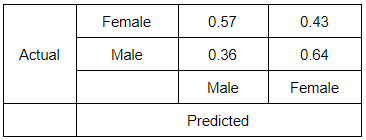
\includegraphics[width=0.7\textwidth]{Images/LR-CM.png}
	\caption{Logistic Regression Model Confusion Matrix}
\end{figure}